\problemname{Backrooms}

The wizard Harry likes to bake.  
One day, he found a spell that could transport him to the ``backrooms'' (this pun only works in Swedish), and he was filled with joy.  
However, when he used the spell, he was not transported to a bakery, but to an infinitely large grid.  
Each cell in the grid is either free or blocked.  
In the grid, you can move up, down, left, or right to adjacent cells that are not blocked.  
After walking around for a while, he notices that the pattern of blocked cells is periodic.  
More precisely, there is an $R \times C$ pattern that repeats infinitely.  
See the figure below for exactly how this works.

\begin{figure}[h]
  \centering
  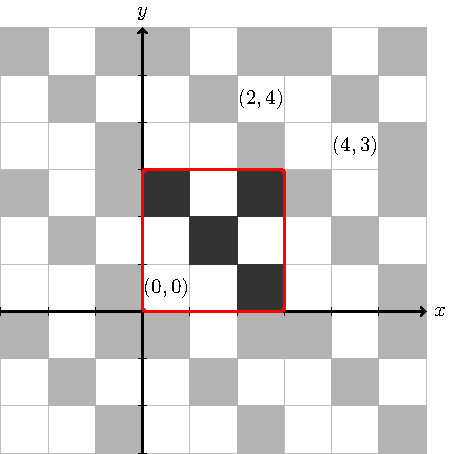
\includegraphics[width=0.4\textwidth]{sampleimage.pdf}
  \caption{Visualization of sample 1. The base pattern is marked in red, and the coordinates of the first question are drawn at $(2,4)$ and $(4,3)$.
  Naturally, the grid continues infinitely beyond what is drawn.}
\end{figure}

To escape, he needs to reach a certain cell in the grid.  
However, his teleportation magic is a bit rusty, so he will ask you five questions of the form:  
``If I teleport to cell $(s_x, s_y)$, can I walk to cell $(g_x, g_y)$?''

\section*{Input}
The first line contains two integers $R$ and $C$ ($1 \leq R,C \leq 5$), the number of rows and columns of the grid.

The next $R$ lines each contain a string of length $C$, consisting of the characters ``\verb|.|'' and ``\verb|#|''.  
These are the rows of the grid. The character ``\verb|#|'' means the cell is blocked, and ``\verb|.|'' means the cell is free.

Then follow five lines.
Each of these lines contains four integers $s_x, s_y, g_x, g_y$ ($0 \leq s_x, s_y, g_x, g_y \leq 10^{12}$), the coordinates for a question.
It is guaranteed that neither of the cells at these are blocked.

\section*{Output}
For every question, print ``\texttt{Ja}'' if Harry can walk from cell $(s_x, s_y)$ to cell $(g_x, g_y)$, otherwise print ``\texttt{Nej}''.

\section*{Scoring}
Your solution will be tested on a set of test groups, each worth a number of points. Each test group contains
a set of test cases. To get the points for a test group you need to solve all test cases in the test group.

\noindent
\begin{tabular}{| l | l | p{12cm} |}
  \hline
  \textbf{Group} & \textbf{Points} & \textbf{Constraints} \\ \hline
  $1$    & $20$  & $R, C \leq 2$ \\ \hline
  $2$    & $20$  & $s_x, s_y, g_x, g_y \leq 500$ \\ \hline
  $3$    & $20$  & $s_x, s_y, g_x, g_y \leq 10^5$ \\ \hline
  $4$    & $40$  & No additional constraints. \\ \hline
\end{tabular}

\section*{Explanation of Sample}
\begin{itemize}
  \item Question 1: Harry starts at $(2,4)$ and wants to move to $(4,3)$.
  To do this, he can move right, down and right.
  \item Question 2: the start and goal are separated by walls, so the answer is ``\texttt{No}''.
  \item Question 3: Harry already starts at the goal, so he is done instantly.
  \item Question 4: even if we are very far out, the grid keeps going. The answer turns out to be ``\texttt{Yes}''.
  \item Question 5: once again, the start and goal are separated by walls.
\end{itemize}

